\chapter{Avancement de la construction système}

\section{Système de vision}

Le framework Open CV est utilisé pour appliquer des filtres et des traitements permettant de détecter le contenu de la carte soit
les îles, les trésors, la station de recharge et la position du robot. La création de fonctions utilitaires de type pipe and filter
permet de tester plus facilement quels filtres sont efficaces et à quel moment, car l'image initiale n'est pas modifiée dans le
traitement. Il est donc possible de voir l'effet de chaque filtre à tout moment. De plus, nous avons créé une configuration
pour les paramètres qui permet de les modifier et de facilement détecter lesquels sont les plus efficaces. Éventuellement, des
tests automatisés seront réalisés avec un grand échantillon d'images afin d'ajouter de la robustesse à nos algorithmes de détection.
Une fois la position des objets détectée, elle est envoyée au robot qui crée la grille utilisée dans la recherche de chemin.


La caméra monde est utilisée au début pour détecter les objets de la carte et construire la grille pour la recherche de chemin. Elle envoie aussi à intervalle régulier la position du robot au robot. La caméra embarquée, quant à elle, est utilisée pour avoir des précisions sur le positionnement précis du robot près de la station de recharge, avant de ramasser le trésor et avant de déposer le trésor.

\section{Tests}
La partie logicielle comporte bien sûr des tests unitaires qui assurent la maintenabilité et la clarté du code.
Les tests fonctionnels quant à eux peuvent être effectués à l'aide d'un simulateur qui remplace ainsi le robot physique.
On peut paramétrer ce simulateur afin qu'il induise du bruit dans le système et soit donc ainsi plus difficile à contrôler.
Ce simulateur est contrôlé par la vraie interface utilisateur du système.
Il suffit de changer le robot dans un fichier de configuration.
Ce fichier de configuration nous permet d'injecter différentes composantes selon le contexte d'exécution.

\section{Interface}
Afin d'obtenir une interface modulaire et la plus polyvalente possible nous avons opté pour une interface web.
Une composante de notre système s'occupe donc de servir les fichiers nécessaires à l'application web.
Celle-ci communique par HTTP REST ou par socket aux autres composantes du système.
La communication par socket est utilisée lorque nous avons besoin d'une boucle de rétroaction rapide,
comme dans le cas de l'information de position du robot.
La section représentant le monde de jeu de l'interface peut afficher beaucoup d'informations.
Afin de ne pas la surcharger, nous avons opté pour que chacun des affichages soit optionnel et puisse donc
être ajouté ou enlevé indépendamment, formant ainsi différentes couches.
Du point de vue des technologies, nous avons utilisé Bootstrap et AngularJS de manière à construire rapidement une interface fonctionnelle.
Pour dessiner les différents éléments de la carte, nous utilisons EaselJS qui nous permet d'utiliser des fonctions avancées de dessin.


\section{Microcontroleur}

Comme interface entre le logiciel et les composantes physiques, nous avons choisi d’utiliser un Arduino Mega 2560. Celui-ci possède une puce différente des autres Arduino, la Atmel2560,
qui permet entre autres d’utiliser plus de de compteur et plus de canaux d’intérruption, fonctionalités qui seront toutes utilisées dans le cadre du projet. Les avantages d’utiliser un Arduino par
rapport à un autre type de microcontroleur sont nombreux. Comme ils sont largement utilisés et qu’ils font partie d’une communauté ouverte, de nombreuses librairies et exemples de toutes sortes sont
disponibles en ligne, permettant de prototyper rapidement différents types de projet. De plus, de nombreuses fonctions de base comme la communication série, les sorties PWM et les entrées ADC sont
prises en charge par la librairie Arduino par défaut.

\section{Communication série}

La communication entre l’ordinateur embarqué et le Mega se fait par communication série.
La librairie PySerial sur Linux et la librairie Serial sur Arduino assure une communication de base simple et efficace. Les communications sont toutes commandées par l’ordinateur embarqué.
Le Mega attend constamment une nouvelle commande à exécuter. Il envoit seulement de l’information sur demande, par exemple le voltage du condensateur de l’électroaimant ou le code manchester.
Pour l’instant, le Arduino peut faire les fonctions suivantes:

\begin{enumerate}

\item move() - permet d’aller dans n’importe direction à la distance et vitesse désirée
\item rotate() -  permet de de tourner avec la direction et l’angle désiré
\item manchester() - retourne par interface série la lettre décodée du code manchester
\item stop() - cesse tout mouvement en cours
\item magnet() - active ou désactive l’alimentation de l’électroaimant
\item lift() - active le préhenseur pour soulever l’aimant
\item capacitor() - retourne par interface série le voltage du condensateur de l’électroaimant
\end{enumerate}

Les fonctions et leurs arguments sont traduits par un décodeur série. Celui-ci interprète les différents octets selon un code préétabli.

\section{Moteurs}

\subsection{Interface moteur}

Chaque moteur est commandé par un canal via le pont H.
Le Arduino se charge d’envoyer les bits de contrôles appropriés à chaque canal selon la commande désirée. Cela permet de contrôler la puissance fournie aux moteurs ainsi
que la direction de rotation. Chaque moteur possède les fonctions suivantes:

\begin{enumerate}
\item set() - Détermine la vitesse désirée, la distance et la direction
\item reset() - Remet tous les paramètres d’un moteur à zéro
\item start() - Démarre le régulateur PID pour un moteur avec les paramètre établis avec le dernier set()
\item brake() - Arrête la roue mais conserve la dernière commande
\end{enumerate}

Également, chaque pair de moteur qui ont la même orientation sont associée par la fonction $move_straight()$. Celle-ci indique au régulateur que ces deux moteurs doivent avoir la même vitesse en tout temps.
Le régulateur va alors constamment regarder la différence de vitesse et de position entre les deux afin de les synchroniser.

\subsection{Régulation des moteurs}

Chaque moteur est régulé principalement en vitesse.
Un timer active le PID à toutes les 50 ms afin de calculer la vitesse de chaque moteur et l’erreur par rapport à la commande.
La sortie est un canal PWM pour chaque moteur qui est envoyé au pont H. Également, lorsqu’une commande $move_straight()$ est appelée, un autre PID cette fois en position est activée afin de
synchroniser les moteurs qui ont la même orientation. Le régulateur arrête automatiquement les moteurs lorsque la distance à parcourir est terminée. L'acquisition de la position des moteurs avec
les encodeurs se fait directement à l’aide de canaux d’interruption qui incrémentent chacun un compteur. La résolution utilisée des encodeurs est de 1600 ticks par révolution de roue, soit le front
 montant d’un seul canal par encodeur.


\subsection{Acquisition du code Manschester}

Le microcontrôleur Arduino Mega sert également à faire la réception du code Manchester. En effet, un récepteur de fréquence radio RF433 est connecté à l’interface série RX1 du microcontrôleur.

Le message provient d’un second Arduino Mega situé à la station de recharge, qui a comme fonction de diffuser en continu le code Manchester. Un transmetteur RF433 compatible avec le
récepteur du robot est donc branché sur l’interface série TX1, diffusant les 32 bits du message sans arrêt, utilisant un protocole série. Aucun traitement n’est fait sur le message par le microcontrôleur.
Il ne fait que l’acquisition et la transmission du message. Cette acquisition se fait à une fréquence de 4.9 kHz. Une synchronisation est effectuée à chaque coup d’horloge afin d’éviter un déphasage.

Les 32 bits du messages sont écrit en continu sur le canal série, avec un baudrate de 1200 Afin d’éviter les erreurs de transmission. Ensuite, lorsque le microcontrôleur du robot reçoit la
commande $manchester()$ par l’ordinateur embarqué, il lit son buffer de réception RX1, qui contient alors les 32 bits du message. Ces bits sont en ordre, mais ne commencent pas nécessairement par le premier.
Ils sont donc lus de manière circulaire, jusqu’à ce que les bits de départ et de fin soient identifiés. Ensuite, ces bits sont décodés selon un encodage Manchester, et le message caché est retourné à
l’ordinateur de base par série.

\subsection{Contrôle de l'électroaimant et du préhenseur}

L’activation de l’électroaimant et du bras préhenseur se fait également par le microcontrôleur embarqué sur le robot. Lorsque l’instruction d’activation de l’électroaimant est reçue, un simple signal
digital 0V-5V est envoyé au module de l’électroaimant. Le courant dans la bobine est ensuite asservi par un régulateur analogique, ce qui évite du travail supplémentaire au microcontrôleur.
Il en est également de même pour le préhenseur: lorsque l’instruction provenant de l’ordinateur de base est reçue, un signal 5V est envoyé au préhenseur.

La tension des condensateurs est également lue par une entrée ADC du microcontroleur. Lors de la recharge des condensateurs, cette tension permet de savoir la progression de la recharge.
Lors du transport du trésor, cette même mesure permet d’estimer le temps restant avant que l’électroaimant n’ait plus de puissance. Puisque la tension des condensateurs est l’un des éléments
à afficher dans l’interface de la station de base, elle peut être transmise par série à l’ordinateur embarqué lorsque la méthode $capacitor()$ est appelée.

\subsection{Contrôle de la caméra}

La caméra embarquée peut tourner sur deux axes à l’aide de servomoteurs HS-422. Ces moteurs sont contrôlés par un Pololu Maestro. Ce microcontrôleur est alimenté par une source de tension 5V,
qui permet également d’alimenter les deux moteurs. Le Pololu est commandé par des commandes séries provenant de l’ordinateur de base, par un câble USB. Afin de faciliter le contrôle des caméras,
une librairie python utilisant PySerial a été conçue. Premièrement, elle reconnait automatiquement sur quel port USB se trouve le Pololu, puis permet de bouger les caméras avec des commandes simples
permettant de bouger la caméra verticalement et horizontalement. La caméra peut être bouger de 180° sur l’axe horizontal et de 90° sur l’angle vertical : il est inutile de regarder vers le haut.
Les commandes ont une précision de 1000 unités par quart de tours, donc de 0.09°. La librairie python permet également de définir une vitesse de mouvement horizontale et verticale, s’il est nécessaire
de faire un mouvement de balayage lent.

\section{Électroaimant}
Le modèle utilisé pour caractérisé l'électroaimant a été très simple. Dans un premier lieu, on a approximé le coeur de fer rond par un transformateur conventionnel. Aussi on s'est limité à l'expression de la force magnétomotrice (FMM) dans le coeur de fer. En effet, les trésors pesent environ 27 g et les moyens dont on dispose peuvent générer des électroaimants qui peuvent soulever des masses largement supérieures. Alors on a observer l'équation de la FMM

\begin{equation}
FMM = NI
\end{equation}

Donc pour produire la FMM, on peut jouer sur le nombre de tours ou le courant qu'on peut injecter dans notre électroaimant. À cause que notre électroaimant est alimenté par une banque de condensateur, il faut maximiser le nombre de tours pour générer la FMM nécessaire afin de limiter le courant pour lever le trésor. Ainsi, on allonge le temps qu'on peut maintenir le trésor. Cependant, mettre un trop grand nombre de tours et la résistance va devenir trop élèvé et on ne sera plus en mesure de lever le trésor. Pour déterminer, le calibre du fils et le nombre de tours, on a calculé dans le Excel, le nombre de tours maximal qu'on peut bobiner par chaque calibre et la résistance résultante. On néglige le comportement dynamique de la bobine, car on est en quasi-statique/statique dans ce problème. Le résultat était du calibre 27 lequel on a bobiné environ 120 tours et on obtient une résistance de $1.23 \Omega$. On peut maintenir le trésor pendant 3 minutes environ avec cet arrangement.

\subsection{Drive de l'électroaimant}

À cause que l'électroaimant va être drivé par un mosfet qui va fonctionner dans la zone de commutation, il faut mettre une diode de roue libre aux bornes de l'électroaimant. On a choisi une diode Schottky à cause de sa grande vitesse de commutation.

  \begin{figure}[H]
    \label{Bobine}
    \centering
    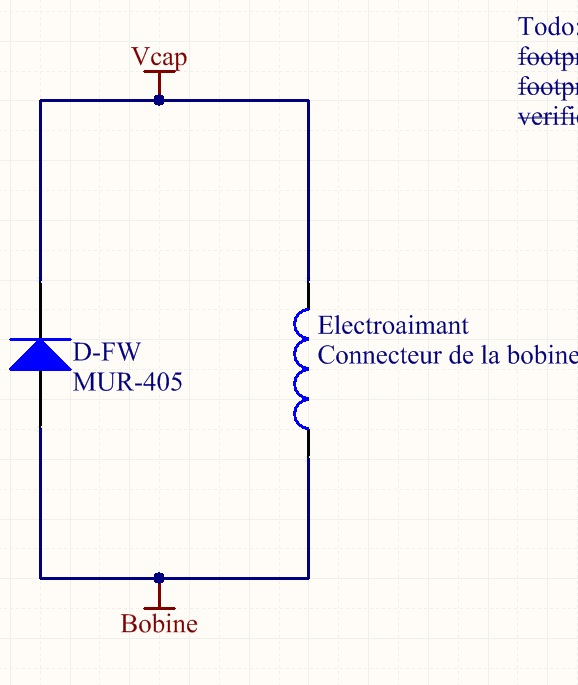
\includegraphics[scale=0.3]{resources/bobine.jpg}
    \caption{Bobine}
  \end{figure}

Afin de mettre du courant dans la bobine, on utilise un MOSFET N-MOS IRF540. Le transistor est commandé par un PWM qui indique la commande de courant dans le transistor. Cette solution a été la première penser à cause de sa très grande simplicité et cette solution a été retenue très rapidement à cause de son bon fonctionnement dans notre application.

  \begin{figure}[H]
    \label{drive}
    \centering
    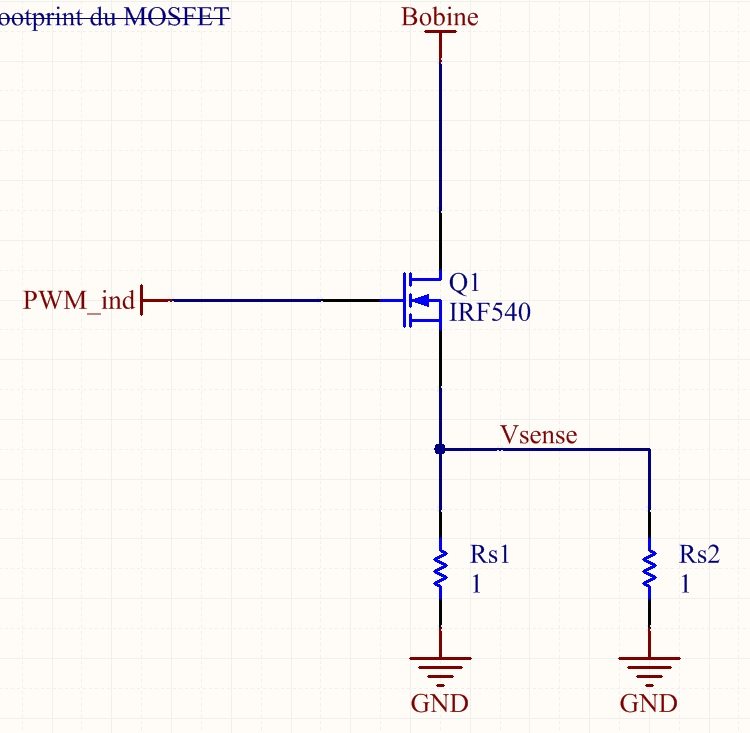
\includegraphics[scale=0.3]{resources/drivemosfet.jpg}
    \caption{Circuit de puissance de la bobine}
  \end{figure}

\subsection{Régulation de l'électroaimant}
Pour maintenir les trésors, il faut avoir un courant constant dans la bobine. Pour ce faire, on avait deux solutions disponible: soit faire un asservissement analogique ou un asservissement numérique avec notre microcontrolleur. L'avantage de l'asservissement numérique est qu'il coûte moins cher en pièce électroniques et qu'on peut facilement changer la commande de courant. En contre-partie, l'asservissement analogique permet de libérer le microcontrolleur qui va être beaucoup solicité par l'asservissement des roues. Donc, après avoir testé, l'asservissement analogique. On a retenue cette solution.

Pour capter le courant, on a mis deux résistance de $1 \Omega$ en parallèle pour obtenir une résistance shunt de $0.5 \Omega$. Ensuite on mesure cette tension à l'aide d'un amplificateur opérationnel (LM358) en mode non-inverseur avec un gain de 10. Finalement, on utilise le second amplificateur opérationnel dans le LM358 pour faire le comparateur avec référence fournit par le microcontrolleur et ainsi générer le PWM qui va commander la Gate du MOSFET.

  \begin{figure}[H]
    \label{drive}
    \centering
    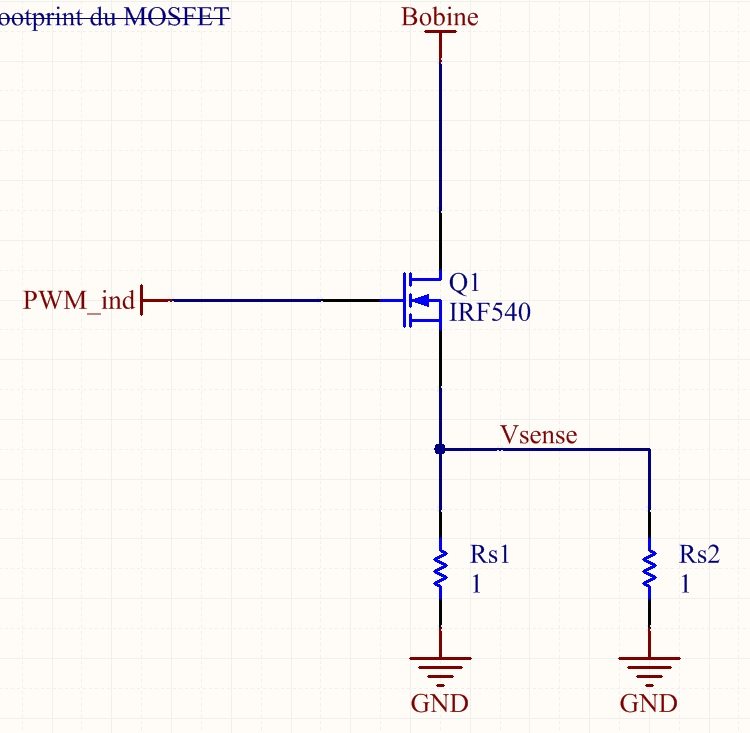
\includegraphics[scale=0.3]{resources/drivemosfet.jpg}
    \caption{Circuit de régulation de la bobine}
  \end{figure}


Pour ajuster la commande du courant, on utilise le trimpot. L'implication de cela est qu'on ne peut pas changer la commande de courant lorsque le robot va être en train de fonctionner, ainsi on met un peu plus de courant pour générer une FMM plus grande au cas où et aussi il faut que les robot s'enligne directement sur les trésors.
\section{Alimentation}

L’alimentation est vitale pour l’accomplissement du robot durant un cycle de jeu. Évidemment, le branchement des régulateurs de tension ne se fait pas directement aux bornes de la batterie. Pour cette raison, il est nécessaire de mettre en place un dispositif qui permet la liaison entre ces deux composantes.

\subsection{Batterie} 

La batterie fournit la puissance nécessaire aux diverses composantes du robot. Une évaluation avec précision de la puissance consommée par le robot ne sera possible que lorsque toutes les composantes seront intégrées. Aussi, ne connaissant pas le comportement du robot en situation de jeux, il est difficile de prévoir la demande en puissance du robot. Avec un manque important d’information à ce niveau, il a été convenu que la batterie doit pouvoir fournir de l’énergie le plus longtemps possible en raison des essais et des tests. De cette manière, il en résultera une meilleure préparation le jour de la compétition.  Ainsi, en considérant la tension nécessaire au régulateur de l’ordinateur embarqué, le choix de la batterie s’est fait selon la consommation maximale de chaque composante du robot. Évidemment, il est peu probable que la demande en puissance de chaque composante soit maximale au même moment, mais cette probabilité n’est pas nul. Il n’a pas eu de tests expérimentalement en lien avec la limite maximale de puissance de chaque composante afin d’éviter tout bris matériel. L’évaluation s’est fait en fonction des informations présentent dans la documentation des appareils. Il en résulte une batterie de type Lipo de 115Wh. Un test élémentaire a été effectué pour obtenir un ordre de grandeur de la chute en tension de la batterie durant l’alimentation de l’ordinateur embarqué s’est avéré concluant. Cette solution assure une alimentation certaine pour la compétition et une durée prolongée pour la préparation.
 
\subsection{Circuit imprimé}

Le circuit imprimé distribue l’énergie de la batterie vers les régulateurs. Sa conception s’est basée sur sa capacité de satisfaire une demande importante en puissance de chaque composante. De plus, le courant délivré par la batterie peut s’avérer dangereux, un fusible s’est avéré incontournable. La largeur des traces a aussi été calculée en fonction du courant pouvant y circuler et l’élévation de température qui en est engendrée. Il en est de même pour les interrupteurs et la grosseur des fils. 



\section{Induction}
\subsection{Alimentation}
Le circuit d'induction partage la même alimentation que celle du module du code manchester soit (5V/3A). 
\subsection{Pont H}
On utilise un pond H afin d'induire un grand courant alternatif dans la bobine du primaire. La fréquence de ce courant est dicté par un PWM généré par le Arduino Uno qui sera aussi situé à la station de base. 

\subsection{Tramsformateur}
Le rapport de transformation entre la bobine primaire et celle du secondaire est d'environ 1:1.2. Ce rapport à été choisi de façon à ce que la bobine du secondaire ait elle aussi un tension d'environ 5V. En effet, le pont H alimenté par du (0-5V) subit une chute de tension de 0.7V causé par les transistors c'est pourquoi il nous faut compenser cet effet par un nombre de tour plus élevée au secondaire qu'au primaire. Pour l'instant, le calibre de fils choisi pour nos deux bobines est le AWG 25, cependant il risque d'être changé lors de lors de l'optimisation.
\subsection{Choix des coeurs de férite}
Afin de facilité l'enlignement des deux bobines, nous avons choisi de prendre des coeurs de férrite de 3,5cm de diamètre. En effet, bien que des coeurs ferrite ayant un diamètre plus petit aurait permit de concentrer d'avantage les lignes de champs magnétique, l'enlignement de ces derniers auraient été un énorme fardeau pour la vision.


\subsection{Circuit d'induction}


  \begin{figure}[H]
    \label{drive}
    \centering
    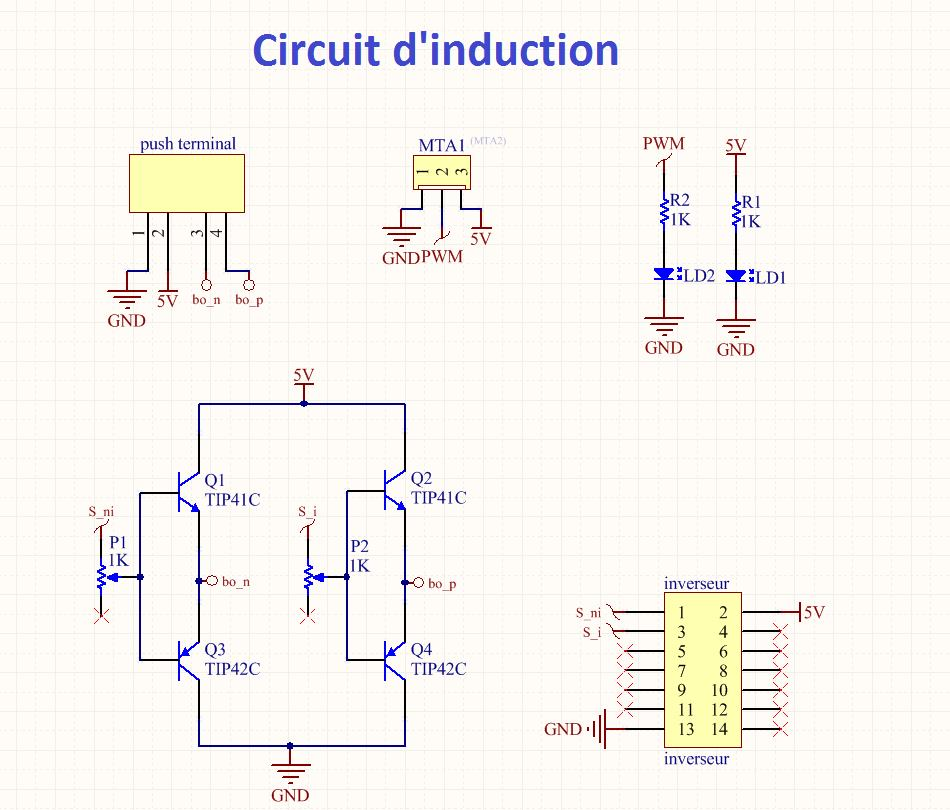
\includegraphics[scale=0.4]{resources/induction.jpg}
    \caption{Circuit d'induction de la bobine}
  \end{figure}

